\documentclass[aspectratio=169]{beamer}
% \usetheme{Madrid}

\usefonttheme{serif}
\setbeamercolor{normal text}{fg=black}

% Make all structural text black (titles, sections, etc.)
\setbeamercolor{structure}{fg=black}

% Frame titles (top title)
\setbeamercolor{frametitle}{fg=black}

% Figure caption ("Figure:")
\setbeamercolor{caption name}{fg=black}
\setbeamercolor{caption}{fg=black}

% Section titles in footer/header
\setbeamercolor{section in head/foot}{fg=black}

% Just in case
\setbeamercolor{title}{fg=black}


% --- Theme setup (minimal) ---
\usetheme{default}
\useoutertheme{default}
\useinnertheme{default}

% Remove navigation symbols
\setbeamertemplate{navigation symbols}{}

% Define your red
% \definecolor{myred}{RGB}{225,120,120}
\definecolor{myred}{RGB}{115,0,10}


\usepackage{color} % color added for editing
\newcommand{\bl}[1]{\textcolor[rgb]{0.00,0.00,1.00}{#1}}
\newcommand{\gr}[1]{\textcolor[rgb]{0.00,0.50,0.00}{#1}}
\newcommand{\rd}[1]{\textcolor[rgb]{0.75,0.00,0.00}{#1}}
\newcommand{\tl}[1]{\textcolor[rgb]{0,0.6,0.60}{#1}}

\usepackage{booktabs}
\usepackage{bm}
\usepackage{mdframed}
\usepackage{xcolor}

% --- Custom footline ---
\setbeamertemplate{footline}{
\leavevmode

% Thin red line (moved to TOP)
\begin{beamercolorbox}[wd=\paperwidth,ht=0.1ex]{}
\color{myred}\rule{\paperwidth}{0.1ex}
\end{beamercolorbox}

\hbox{
\begin{beamercolorbox}[wd=\paperwidth,ht=2.5ex,dp=1ex]{}
\hspace{1em}
\insertsection
\hfill
\insertframenumber{} / \inserttotalframenumber
\hspace{1em}
\end{beamercolorbox}
}
}

% Remove headline entirely
\setbeamertemplate{headline}{}

% Optional: clean fonts
\setbeamerfont{footline}{size=\small}







\title{Chapter~4~Classification}
\author{Austin R.J. Downey}
\date{}

\begin{document}

\section{Machine Learning for Engineering Problem Solving}
\frame{\titlepage}


\section{Chapter~4~Machine Learning Workflows}

\section{4.1~Binary Classifier}


%------------------------------------------------

\begin{frame}{Classification}
	\begin{columns}
		
		\column{0.45\textwidth}
		
		Machine learning tasks often fall into two categories:
		
		\vspace{0.5em}
		
		\begin{itemize}
			\item Regression
			\begin{itemize}
				\item Predict continuous values
			\end{itemize}
			
			\vspace{0.3em}
			
			\item Classification
			\begin{itemize}
				\item Predict discrete classes
			\end{itemize}
		\end{itemize}
		
		\vspace{0.5em}
		
		In this chapter we focus on:
		
		\begin{itemize}
			\item Binary classification
			\item Multiclass classification
			\item Performance metrics
		\end{itemize}
		
		\column{0.55\textwidth}
		\centering
		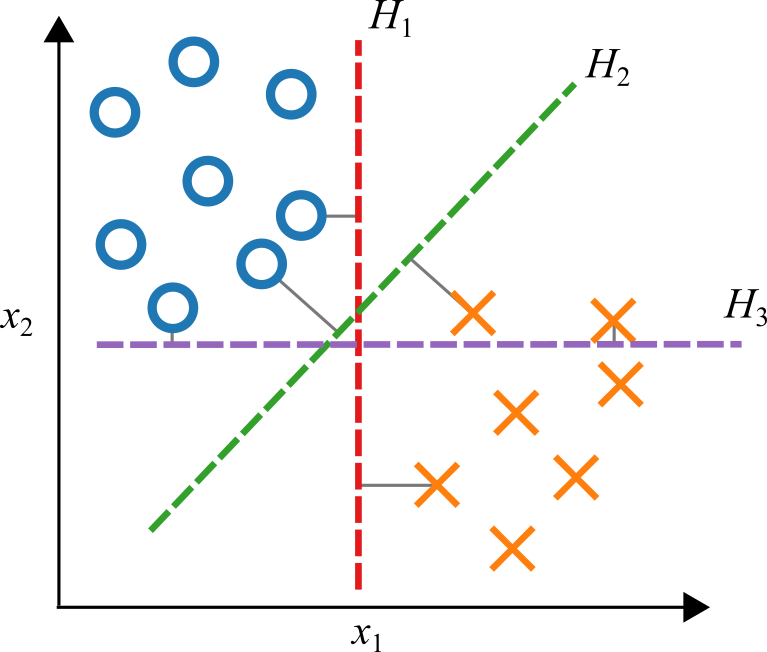
\includegraphics[width=\textwidth]
		{../figures/x_y_plot_linear_classifier}
		
		\vspace{0.3em}
		{\small Linear decision boundaries separating two classes.}
		
	\end{columns}
\end{frame}

%------------------------------------------------

\begin{frame}{Binary Classifier}
	\begin{columns}
		
		\column{0.48\textwidth}
		
		A binary classifier assigns inputs to one of two classes.
		
		\vspace{0.5em}
		
		Decision rule:
		
		\[
		\hat{y}
		=
		\begin{cases}
			1 & \text{if }\bm{\theta}^{\top}\mathbf{x}+b \ge 0 \\
			0 & \text{otherwise}
		\end{cases}
		\]
		
		\vspace{0.5em}
		
		\begin{itemize}
			\item $\mathbf{x}$: input features
			\item $\bm{\theta}$: model weights
			\item $b$: bias term
		\end{itemize}
		
		\vspace{0.5em}
		
		Training adjusts $\bm{\theta}$ and $b$ to minimize classification error.
		
		\column{0.52\textwidth}
		\centering
		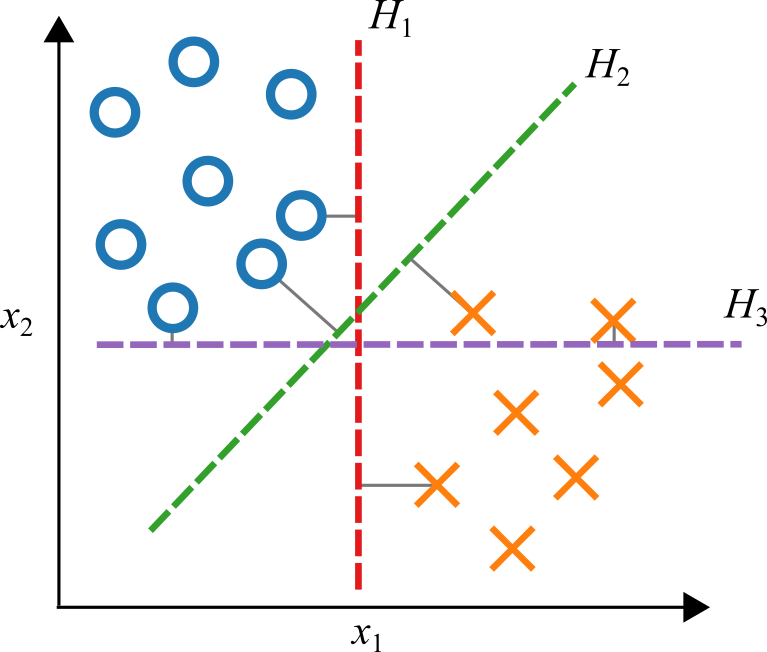
\includegraphics[width=\textwidth]
		{../figures/x_y_plot_linear_classifier}
		
		\vspace{0.3em}
		{\small Multiple linear decision boundaries can correctly separate the data.}
		
	\end{columns}
\end{frame}

%------------------------------------------------

\begin{frame}{Data: MNIST Dataset}
	\begin{columns}
		
		\column{0.48\textwidth}
		
		The MNIST dataset contains:
		
		\begin{itemize}
			\item 70,000 handwritten digits
			\item Classes 0 through 9
			\item Standard benchmark for classification
		\end{itemize}
		
		\vspace{0.5em}
		
		Typical split:
		
		\begin{itemize}
			\item 60,000 training images
			\item 10,000 testing images
		\end{itemize}
		
		\column{0.52\textwidth}
		\centering
		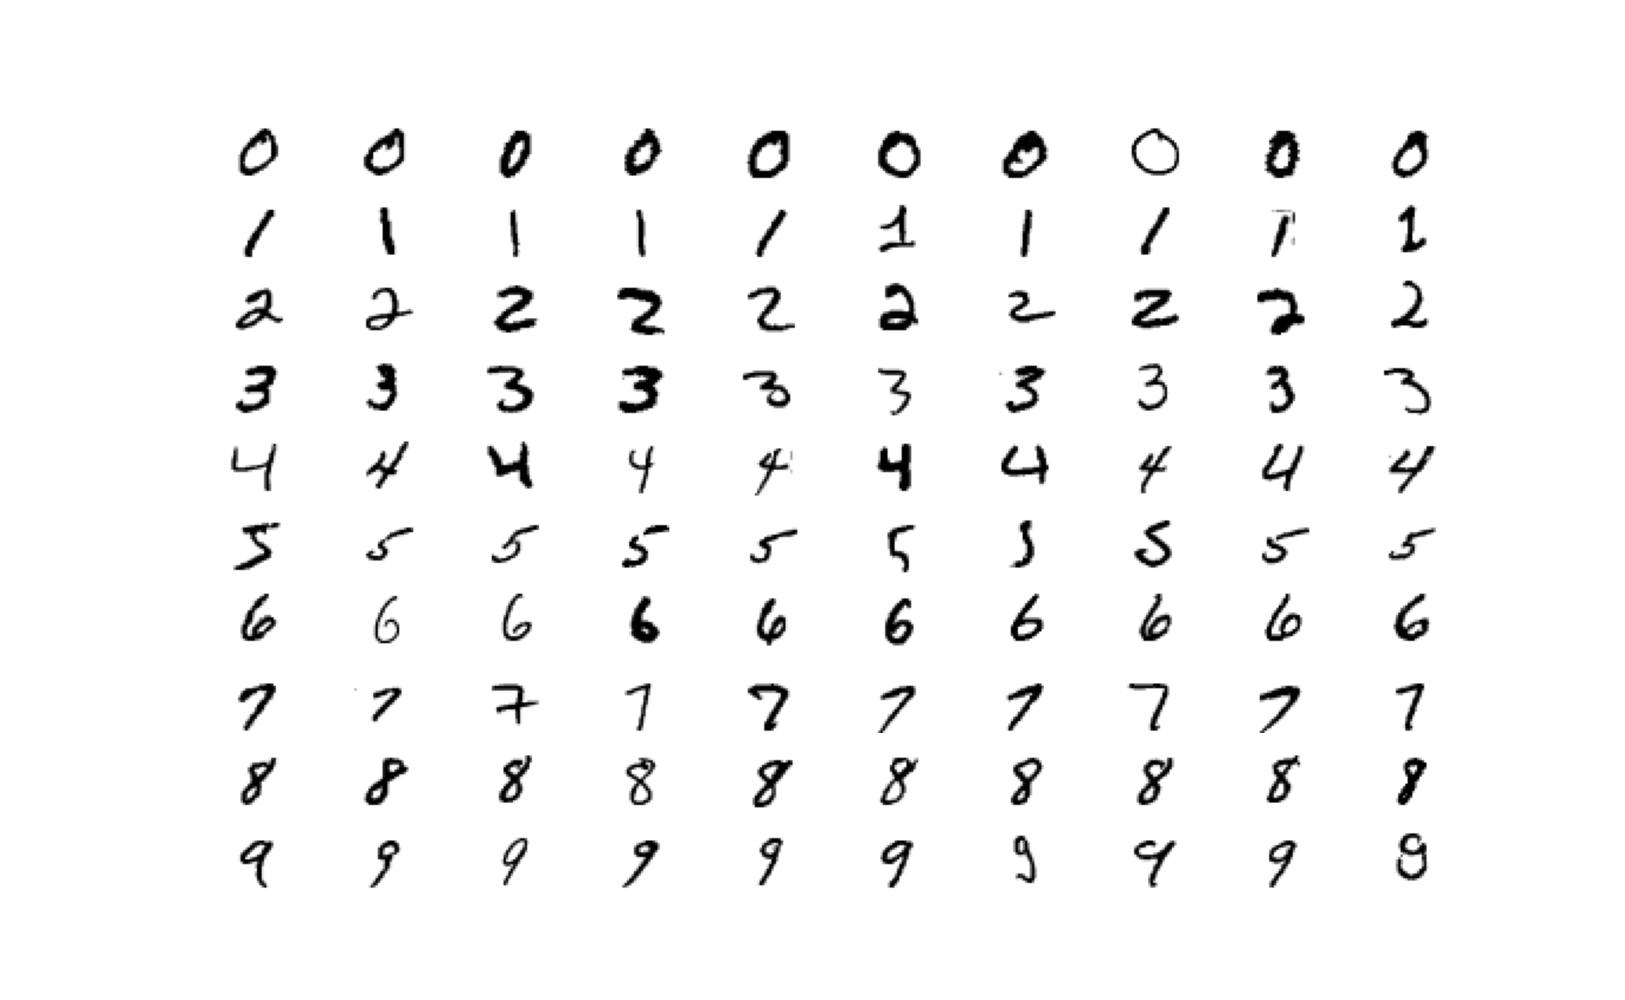
\includegraphics[width=\textwidth]
		{../figures/MNIST_data_set}
		
		\vspace{0.3em}
		{\small Examples of MNIST digits.}
		
	\end{columns}
\end{frame}

%------------------------------------------------

\begin{frame}{Data: What is a Feature?}
	\begin{columns}
		
		\column{0.48\textwidth}
		
		Each MNIST image is:
		
		\[
		28 \times 28 = 784
		\]
		
		pixels.
		
		\vspace{0.5em}
		
		In machine learning:
		
		\begin{itemize}
			\item Each pixel is a feature
			\item Pixel intensity ranges from 0 to 255
			\item One image becomes a vector with 784 features
		\end{itemize}
		
		\vspace{0.5em}
		
		For MNIST:
		
		\[
		\mathbf{x}
		=
		[x_1,x_2,\ldots,x_{784}]
		\]
		
		\column{0.52\textwidth}
		\centering
		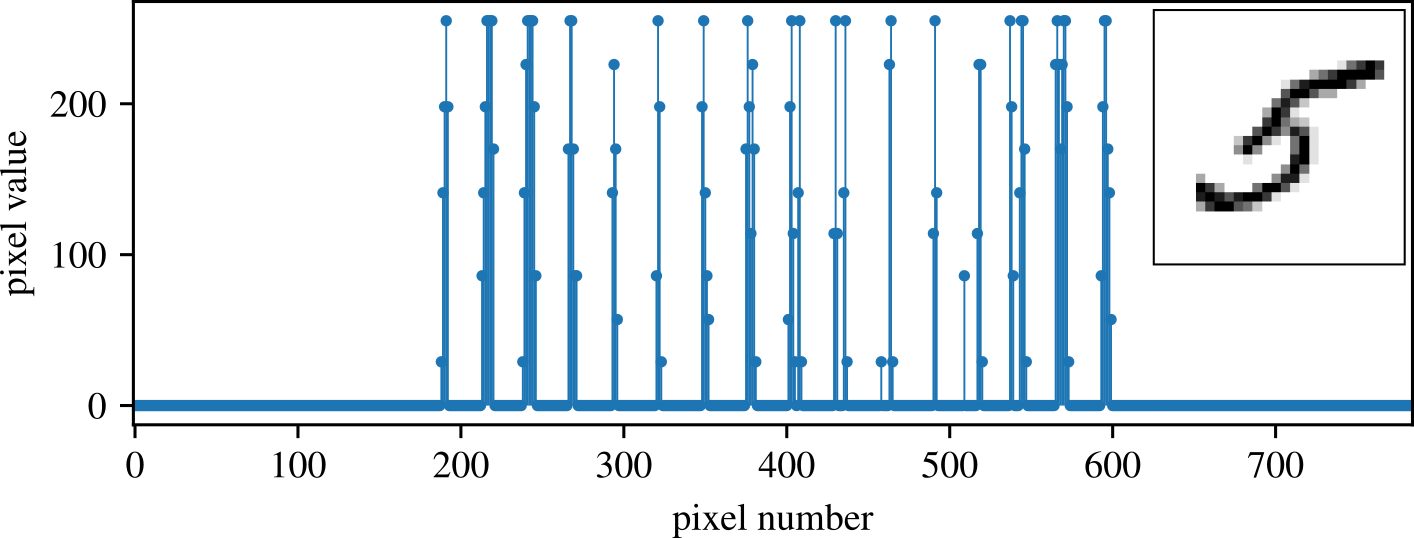
\includegraphics[width=\textwidth]
		{../figures/MNIST_digit_features}
		
		\vspace{0.3em}
		{\small Each pixel becomes a feature used by the classifier.}
		
	\end{columns}
\end{frame}

%------------------------------------------------

\begin{frame}{Example 4.1: MNIST Dataset}
	
	To simplify the classification problem, we begin by building a: \textbf{5-detector}
	
	\vspace{0.5em}
	
	Goal:
	\begin{itemize}
		\item Determine whether a digit is a 5
		\item Binary output:
		\begin{itemize}
			\item 1 = digit is a 5
			\item 0 = digit is not a 5
		\end{itemize}
	\end{itemize}
	
	\vspace{0.5em}
	
	Why choose 5s?
	
	\begin{itemize}
		\item One of the most difficult digits to classify
		\item Frequently confused with 3s and 8s
		\item Good benchmark for binary classification
	\end{itemize}
	
	\vspace{0.5em}
	
	This example demonstrates how to use:
	
	\[
	\texttt{sklearn.datasets.fetch\_openml}
	\]
	
	to load and visualize the MNIST dataset.
	
\end{frame}

%------------------------------------------------

\begin{frame}{Regularized Linear Classifier}
	
	A practical way to build the MNIST ``5-detector'' is with a regularized linear classifier trained using Stochastic Gradient Descent.
	
	\vspace{0.5em}
	
	\begin{itemize}
		\item Efficient on large datasets
		\item Simple to implement
		\item Updates one example at a time
	\end{itemize}
	
	\vspace{0.5em}
	
	Main drawbacks:
	\begin{itemize}
		\item Needs careful hyperparameter tuning
		\item Sensitive to feature scaling
	\end{itemize}
	
\end{frame}

%------------------------------------------------

\begin{frame}{Training Objective}
	
	Given labeled samples $(\mathbf{x}^{(i)}, y^{(i)})$ with $y^{(i)} \in \{0,1\}$, the ``5-detector'' learns parameters by minimizing:
	
	\[
	J(\boldsymbol{\theta}) =
	\frac{1}{m}\sum_{i=1}^{m}
	\max\bigl(0, 1 - y^{(i)}\boldsymbol{\theta}^{\text{T}}\mathbf{x}^{(i)}\bigr)
	+
	\frac{\lambda}{2}\,\lVert \boldsymbol{\theta}_{1:} \rVert_2^2
	\]
	
	\vspace{0.5em}
	
	\begin{itemize}
		\item First term: hinge loss
		\item Second term: $\ell_2$ regularization
		\item Bias term is not regularized
	\end{itemize}
	
	\begin{exampleblock}{Note}
		In scikit-learn, this model is implemented as \texttt{SGDClassifier}.
	\end{exampleblock}
	
\end{frame}

%------------------------------------------------

\begin{frame}{Example 4.2: Regularized Linear Classifier}
	
	\begin{itemize}
		\item Train a regularized linear classifier with \texttt{SGDClassifier}
		\item Use the MNIST dataset to distinguish the digit ``5'' from all others
		\item Show how regularization improves generalization
		\item Demonstrate prediction on a selected handwritten digit
	\end{itemize}
	
	\vspace{0.5em}
	
	This example illustrates how a sparse linear decision boundary can work well for binary digit classification.
	
\end{frame}

%------------------------------------------------

\section{4.2~Performance Measures for Binary Classification}

\begin{frame}{Performance Measures for Classification}
	
	Evaluating a classifier is often more challenging than evaluating a regressor.
	
	\vspace{0.5em}
	
	Questions we might ask:
	
	\begin{itemize}
		\item How many predictions were correct?
		\item What kinds of mistakes were made?
		\item Which classes are most often confused?
	\end{itemize}
	
	\vspace{0.5em}
	
	A common tool for answering these questions is the:
	
	\[
	\textbf{Confusion Matrix}
	\]
	
\end{frame}

%------------------------------------------------

\begin{frame}{Binary Confusion Matrix}
	\begin{columns}
		
		\column{0.48\textwidth}
		
		Two common error types:
		
		\vspace{0.5em}
		
		\begin{itemize}
			\item Type I Error:
			\begin{itemize}
				\item False Positive (FP)
			\end{itemize}
			
			\vspace{0.3em}
			
			\item Type II Error:
			\begin{itemize}
				\item False Negative (FN)
			\end{itemize}
		\end{itemize}
		
		\vspace{0.5em}
		
		A confusion matrix summarizes:
		
		\begin{itemize}
			\item True Positives (TP)
			\item True Negatives (TN)
			\item False Positives (FP)
			\item False Negatives (FN)
		\end{itemize}
		
		\column{0.52\textwidth}
		\centering
		
\includegraphics[width=\textwidth]
		{../figures/confusion_matrix_binary.png}
		
		\vspace{0.3em}
		{\small Binary confusion matrix.}
		
	\end{columns}
\end{frame}

%------------------------------------------------

\begin{frame}{Confusion Matrix}
	\begin{columns}
		
		\column{0.48\textwidth}
		
		Rows correspond to:
		
		\begin{itemize}
			\item Actual classes
		\end{itemize}
		
		\vspace{0.5em}
		
		Columns correspond to:
		
		\begin{itemize}
			\item Predicted classes
		\end{itemize}
		
		\vspace{0.5em}
		
		A good classifier has:
		
		\begin{itemize}
			\item Large values on the diagonal
			\item Small values elsewhere
		\end{itemize}
		
		\vspace{0.5em}
		
		Off-diagonal entries indicate misclassifications.
		
		\column{0.52\textwidth}
		\centering
		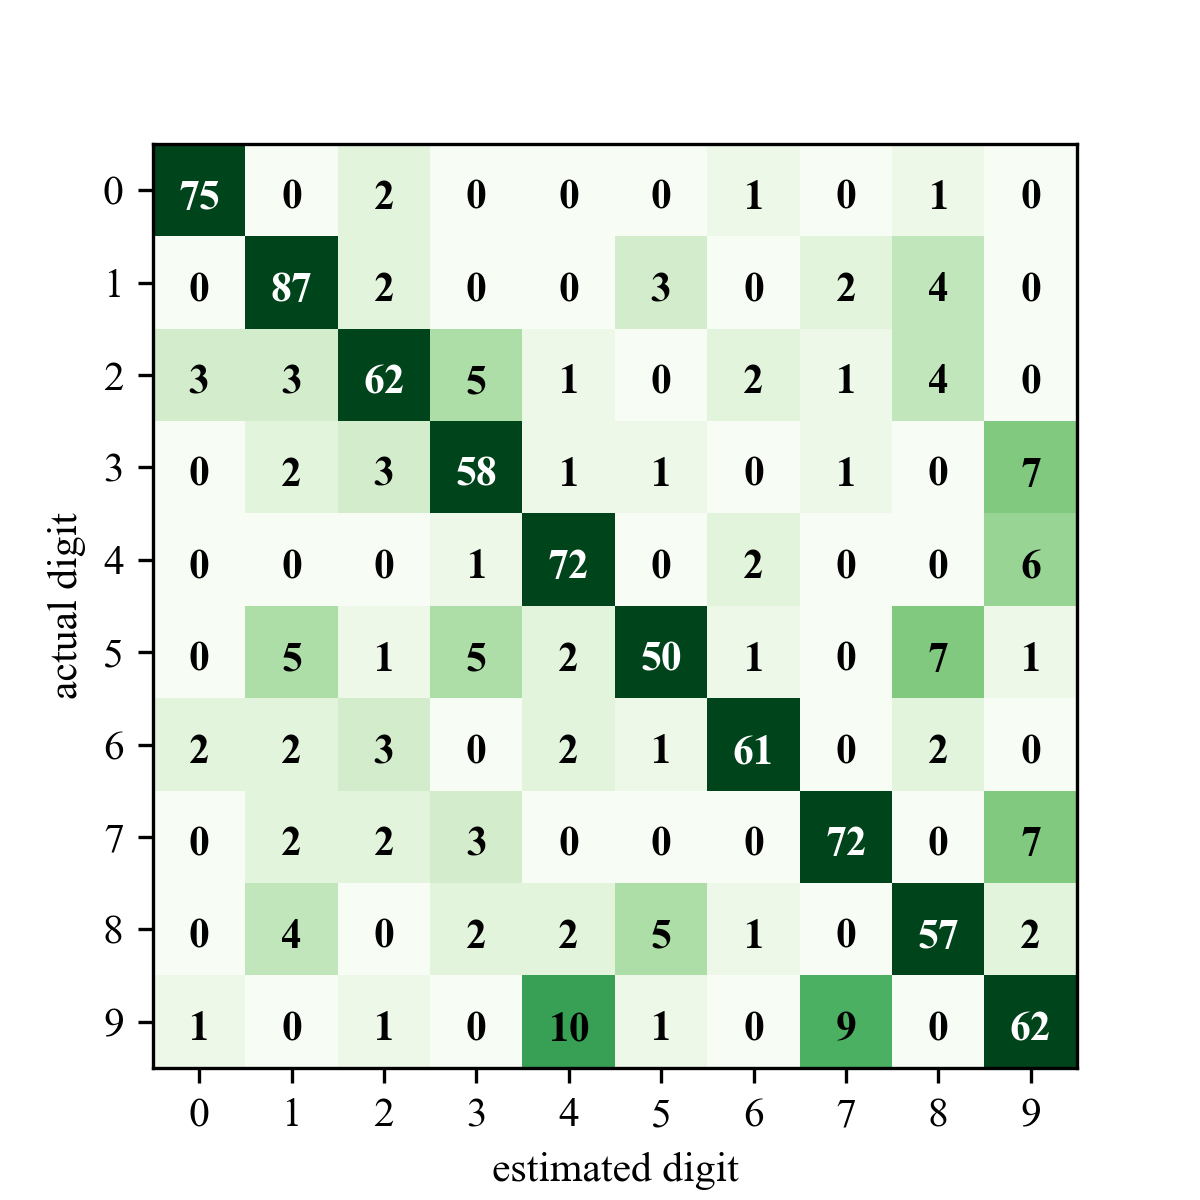
\includegraphics[width=0.9\textwidth]
		{../figures/digit_confusion_matrix_limited.png}
		
		\vspace{0.3em}
		{\small MNIST confusion matrix.}
		
	\end{columns}
\end{frame}

%------------------------------------------------

\begin{frame}{Confusion Matrix Terminology}
	\begin{columns}
		
		\column{0.40\textwidth}
		
		A confusion matrix summarizes classifier predictions.
		
		\vspace{0.5em}
		
		\begin{itemize}
			\item Rows = actual class
			\item Columns = predicted class
		\end{itemize}
		
		\vspace{0.5em}
		
		\begin{itemize}
			\item TP: True Positive
			\item TN: True Negative
			\item FP: False Positive
			\item FN: False Negative
		\end{itemize}
		
		\vspace{0.5em}
		
		A perfect classifier contains values only along the main diagonal.
		
		\column{0.60\textwidth}
		\centering
		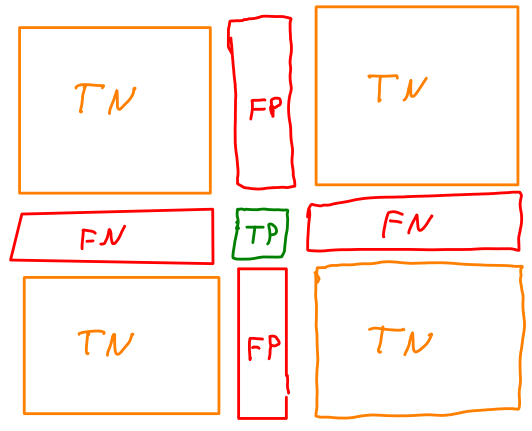
\includegraphics[width=\textwidth]
		{../figures/confusion_matrix_breakout.png}
		
	\end{columns}
\end{frame}

%------------------------------------------------

\begin{frame}{Example 4.3: Binary Confusion Matrix}
	
	\begin{itemize}
		\item Train a binary classifier to detect the digit ``5''
		\item Generate a confusion matrix
		\item Compute:
		\begin{itemize}
			\item True Positives (TP)
			\item True Negatives (TN)
			\item False Positives (FP)
			\item False Negatives (FN)
		\end{itemize}
		
		\vspace{0.5em}
		
		\item Examine examples of:
		\begin{itemize}
			\item Missed 5s (false negatives)
			\item Incorrectly detected 5s (false positives)
		\end{itemize}
		
		\vspace{0.5em}
		
		\item Use the confusion matrix to understand where the classifier fails
	\end{itemize}
	
\end{frame}

%------------------------------------------------

\begin{frame}{Accuracy}
	
	Accuracy is defined as
	
	\[
	\text{Accuracy}
	=
	\frac{\text{Correct Predictions}}
	{\text{Total Predictions}}
	\]
	
	or
	
	\[
	\text{Accuracy}
	=
	\frac{TP+TN}
	{TP+TN+FP+FN}
	\]
	
	\vspace{0.5em}
	
	\begin{itemize}
		\item Simple and intuitive
		\item Often the first metric reported
		\item Does not distinguish between error types
	\end{itemize}
	
\end{frame}

%------------------------------------------------

\begin{frame}{Why Accuracy Isn't Enough}
	
	A classifier may achieve high accuracy while still making costly mistakes.
	
	\vspace{0.5em}
	
	Examples:
	
	\begin{itemize}
		\item Credit card fraud detection
		\item Medical diagnosis
		\item Network intrusion detection
	\end{itemize}
	
	\vspace{0.5em}
	
	A false negative may be much more costly than a false positive.
	
	\vspace{0.5em}
	
	We therefore introduce:
	
	\[
	\textbf{Precision}
	\qquad
	\textbf{Recall}
	\]
	
\end{frame}

%------------------------------------------------

\begin{frame}{Selected and Relevant Instances}
	\begin{columns}
		
		\column{0.48\textwidth}
		
		Definitions:
		
		\[
		\text{Selected Instances}
		=
		TP+FP
		\]
		
		\[
		\text{Relevant Instances}
		=
		TP+FN
		\]
		
		\vspace{0.5em}
		
		These quantities form the basis of precision and recall.
		
		\column{0.52\textwidth}
		\centering
		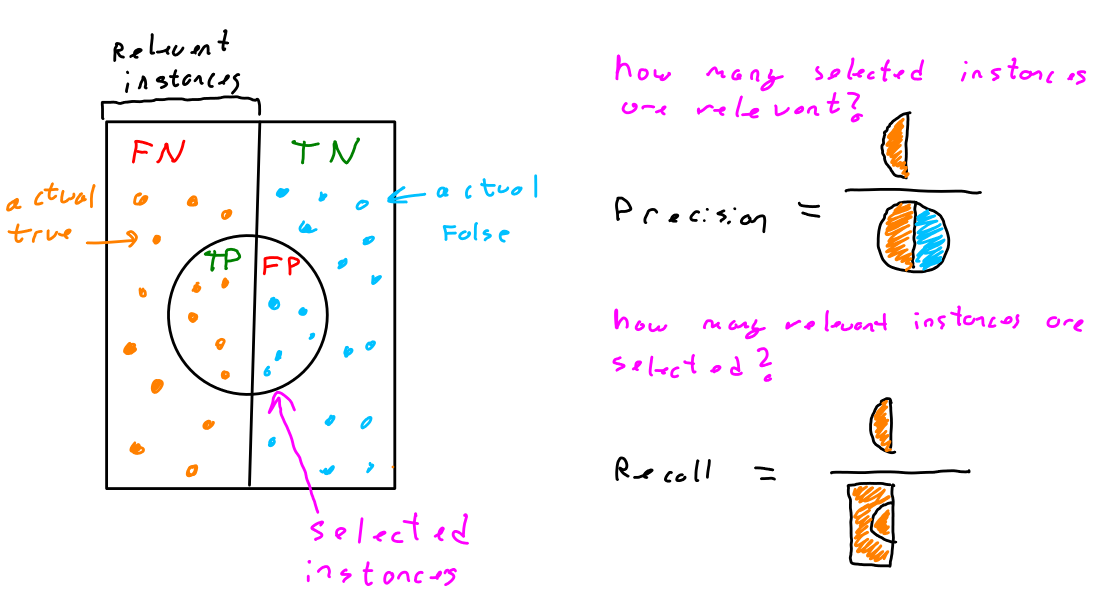
\includegraphics[width=\textwidth]
		{../figures/piechart_TP_vs_FP.png}
		
	\end{columns}
\end{frame}

%------------------------------------------------

\begin{frame}{Precision}
	
	Precision answers:
	
	\vspace{0.3em}
	
	\emph{Of all positive predictions, how many were correct?}
	
	\vspace{0.5em}
	
	\[
	\text{Precision}
	=
	\frac{TP}
	{TP+FP}
	\]
	
	\vspace{0.5em}
	
	High precision implies:
	
	\begin{itemize}
		\item Few false positives
		\item Positive predictions are trustworthy
	\end{itemize}
	
\end{frame}

%------------------------------------------------

\begin{frame}{Recall}
	
	Recall answers:
	
	\vspace{0.3em}
	
	\emph{Of all actual positives, how many were found?}
	
	\vspace{0.5em}
	
	\[
	\text{Recall}
	=
	\frac{TP}
	{TP+FN}
	\]
	
	\vspace{0.5em}
	
	High recall implies:
	
	\begin{itemize}
		\item Few false negatives
		\item Important cases are not missed
	\end{itemize}
	
\end{frame}

%------------------------------------------------

\begin{frame}{F1 Score}
	
	The F1 score balances precision and recall.
	
	\[
	F_1
	=
	2
	\frac{\text{Precision}\times\text{Recall}}
	{\text{Precision}+\text{Recall}}
	\]
	
	\vspace{0.5em}
	
	Equivalent form:
	
	\[
	F_1
	=
	\frac{TP}
	{TP+\frac{FP+FN}{2}}
	\]
	
	\vspace{0.5em}
	
	Useful when both precision and recall are important.
	
\end{frame}

%------------------------------------------------

\begin{frame}{Precision--Recall Tradeoff}
	\begin{columns}
		
		\column{0.48\textwidth}
		
		Changing the classification threshold changes:
		
		\begin{itemize}
			\item Precision
			\item Recall
			\item F1 score
		\end{itemize}
		
		\vspace{0.5em}
		
		Higher threshold:
		
		\begin{itemize}
			\item Higher precision
			\item Lower recall
		\end{itemize}
		
		\column{0.52\textwidth}
		\centering
		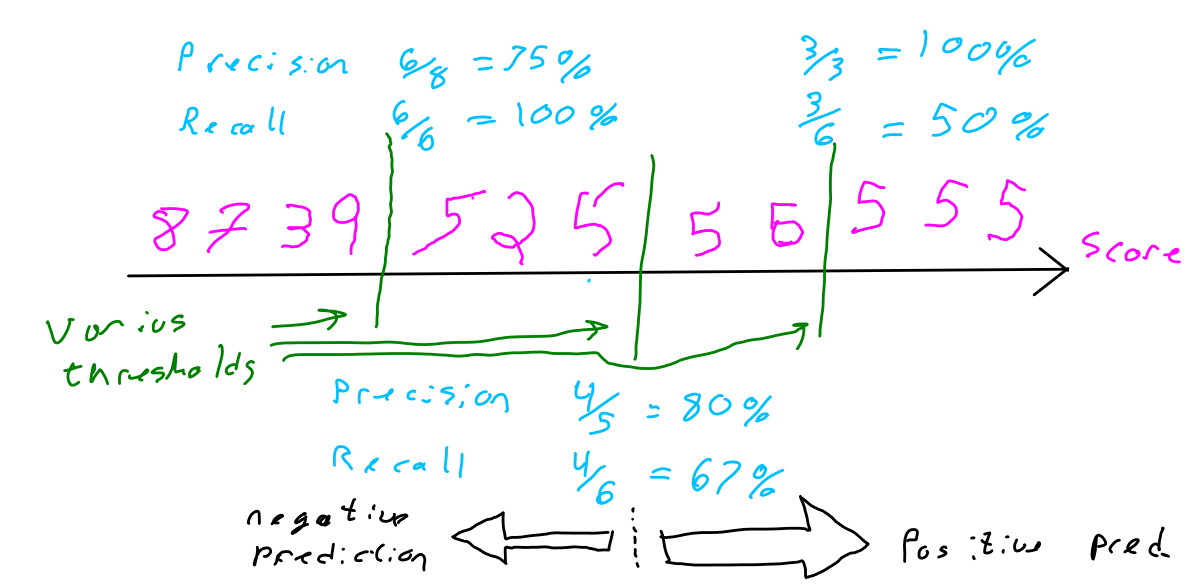
\includegraphics[width=\textwidth]
		{../figures/decision_threshold.png}
		
	\end{columns}
\end{frame}

%------------------------------------------------

\begin{frame}{Choosing a Threshold}
	\begin{columns}
		
		\column{0.48\textwidth}
		
		Threshold selection depends on the application.
		
		\vspace{0.5em}
		
		Examples:
		
		\begin{itemize}
			\item Medical diagnosis $\rightarrow$ high recall
			\item Spam detection $\rightarrow$ high precision
		\end{itemize}
		
		\vspace{0.5em}
		
		The F1 score often helps identify a good compromise.
		
		\column{0.52\textwidth}
		\centering
		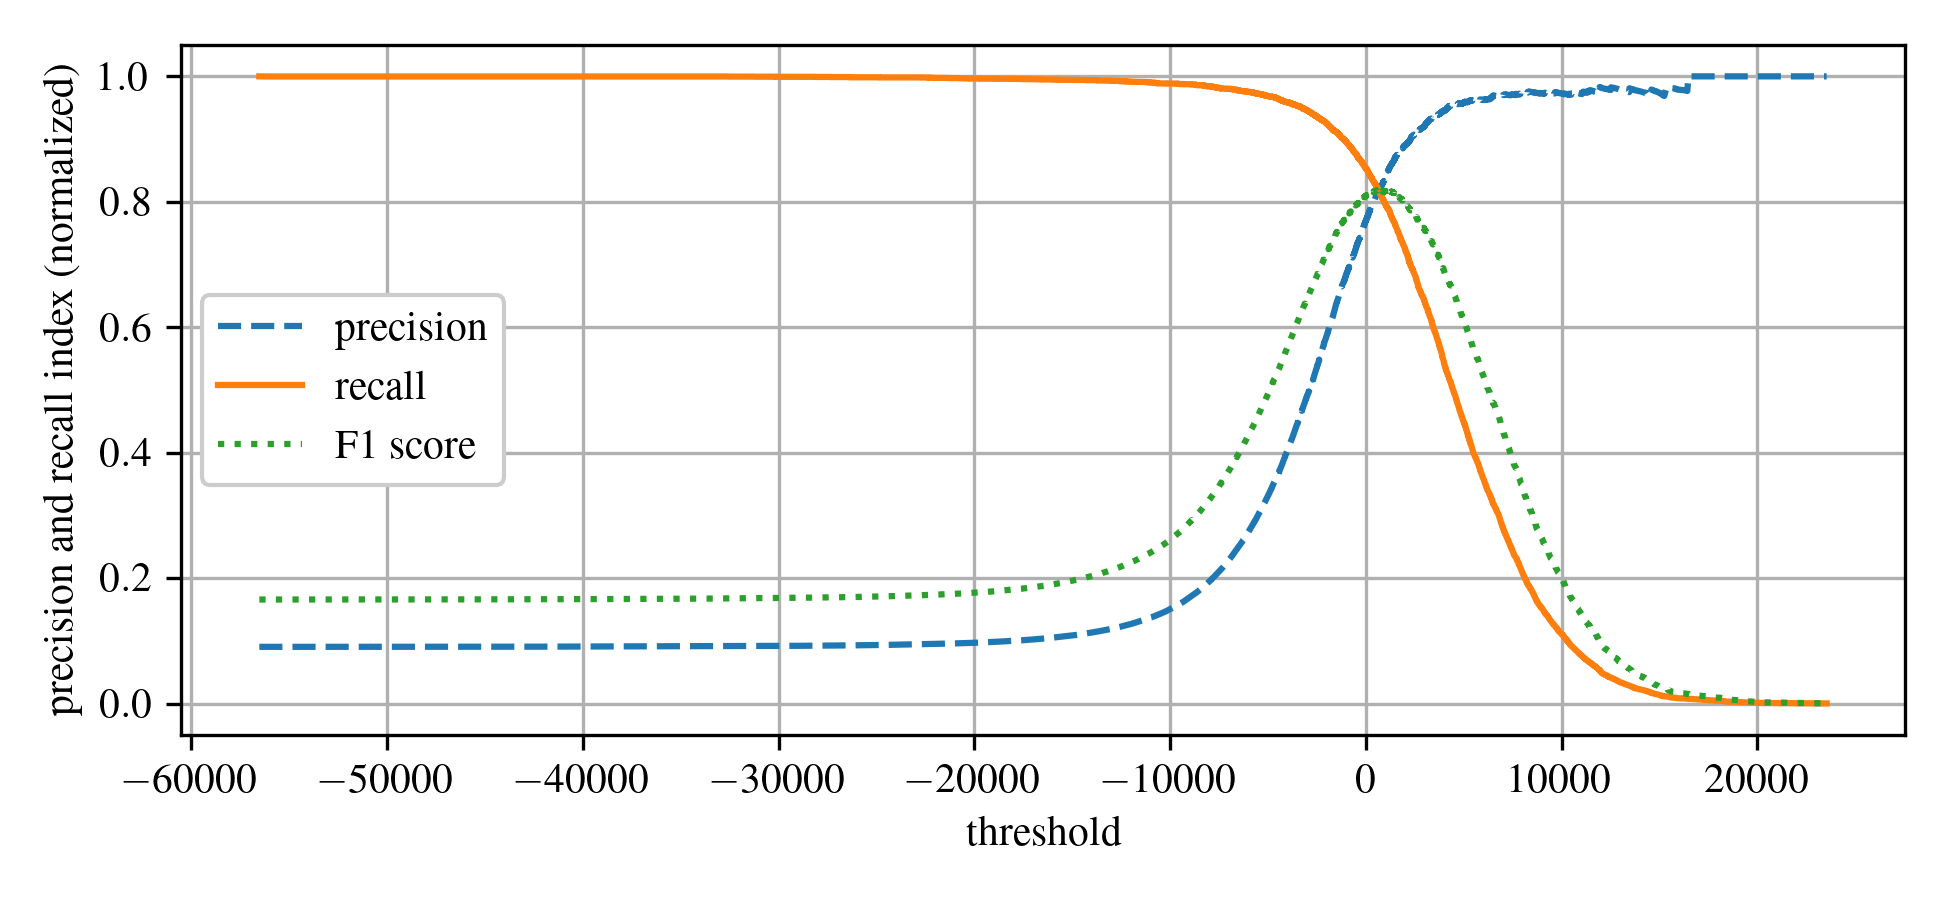
\includegraphics[width=\textwidth]
		{../figures/F1_score_plot.png}
		
	\end{columns}
\end{frame}

%------------------------------------------------

\begin{frame}{Precision--Recall Curve}
	\begin{columns}
		
		\column{0.48\textwidth}
		
		The precision--recall curve summarizes classifier performance across all thresholds.
		
		\vspace{0.5em}
		
		Better classifiers typically have:
		
		\begin{itemize}
			\item Higher precision
			\item Higher recall
			\item Larger AUC-PR
		\end{itemize}
		
		\vspace{0.5em}
		
		Applications determine the desired operating point.
		
		\column{0.52\textwidth}
		\centering
		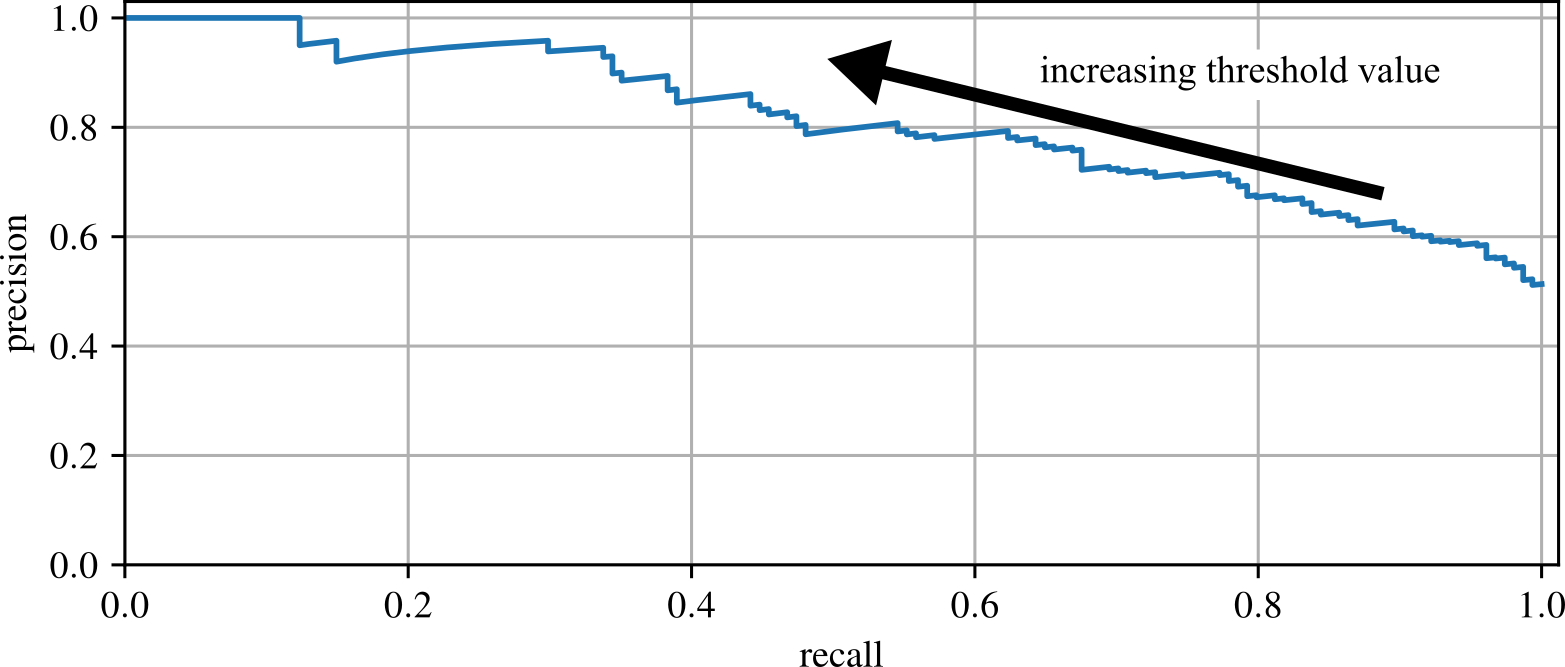
\includegraphics[width=\textwidth]
		{../figures/precision_recall_curve}
		
	\end{columns}
\end{frame}

%------------------------------------------------

\begin{frame}{Example 4.4: Accuracy, Precision, and Recall}
	
	\begin{itemize}
		\item Train a binary classifier to detect the digit ``5''
		\item Compute:
		\begin{itemize}
			\item Accuracy
			\item Precision
			\item Recall
			\item F1 Score
		\end{itemize}
		
		\vspace{0.5em}
		
		\item Compare manual and sklearn calculations
		\item Visualize threshold effects
		\item Explore precision--recall tradeoffs
	\end{itemize}
	
\end{frame}

%------------------------------------------------

\section{4.3~$k$-fold Cross-validation}

%------------------------------------------------

\begin{frame}{$k$-fold Cross-Validation}
	
	Training an SGD classifier does not always produce identical results.
	
	\vspace{0.5em}
	
	Reasons:
	
	\begin{itemize}
		\item Random initialization
		\item Random ordering of samples
		\item Stochastic optimization
	\end{itemize}
	
	\vspace{0.5em}
	
	Possible solutions:
	
	\begin{itemize}
		\item More training epochs
		\item More data
		\item Cross-validation
	\end{itemize}
	
	\vspace{0.5em}
	
	Goal:
	\begin{itemize}
		\item Obtain a more reliable estimate of model performance
	\end{itemize}
	
\end{frame}

%------------------------------------------------

\begin{frame}{Performance Variability}
	\begin{columns}
		
		\column{0.48\textwidth}
		
		Repeated training can produce different results.
		
		\vspace{0.5em}
		
		Observations:
		
		\begin{itemize}
			\item Accuracy varies
			\item Precision varies
			\item Recall varies
		\end{itemize}
		
		\vspace{0.5em}
		
		Cross-validation reduces this variability and produces more stable estimates.
		
		\column{0.52\textwidth}
		\centering
		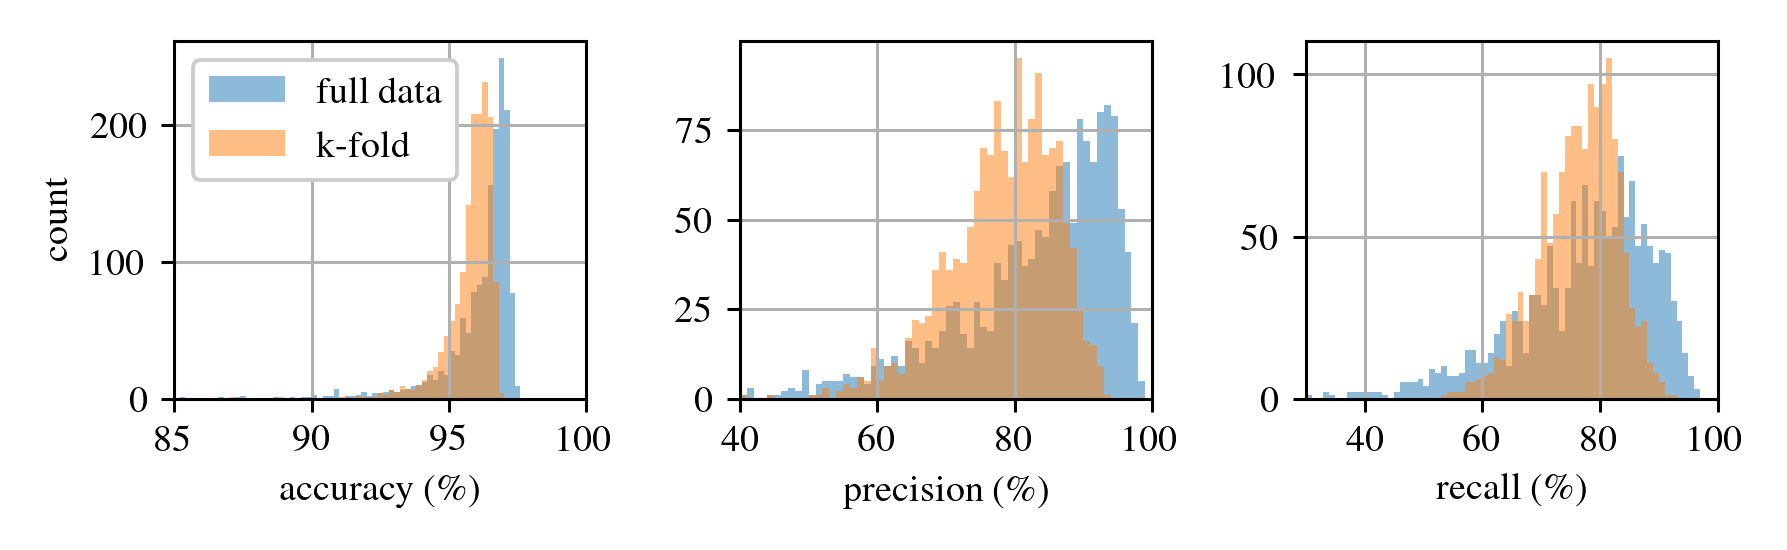
\includegraphics[width=\textwidth]
		{../figures/k-fold_cross-validation_trials}
		
	\end{columns}
\end{frame}

%------------------------------------------------

\begin{frame}{How $k$-fold Cross-Validation Works}
	\begin{columns}
		
		\column{0.48\textwidth}
		
		Procedure:
		
		\begin{enumerate}
			\item Split data into $k$ folds
			\item Train on $k-1$ folds
			\item Validate on the remaining fold
			\item Repeat for all folds
			\item Average the results
		\end{enumerate}
		
		\vspace{0.5em}
		
		Advantages:
		
		\begin{itemize}
			\item Uses all available data
			\item Better estimate of performance
			\item Reduces dependence on a single train/test split
		\end{itemize}
		
		\column{0.52\textwidth}
		\centering
		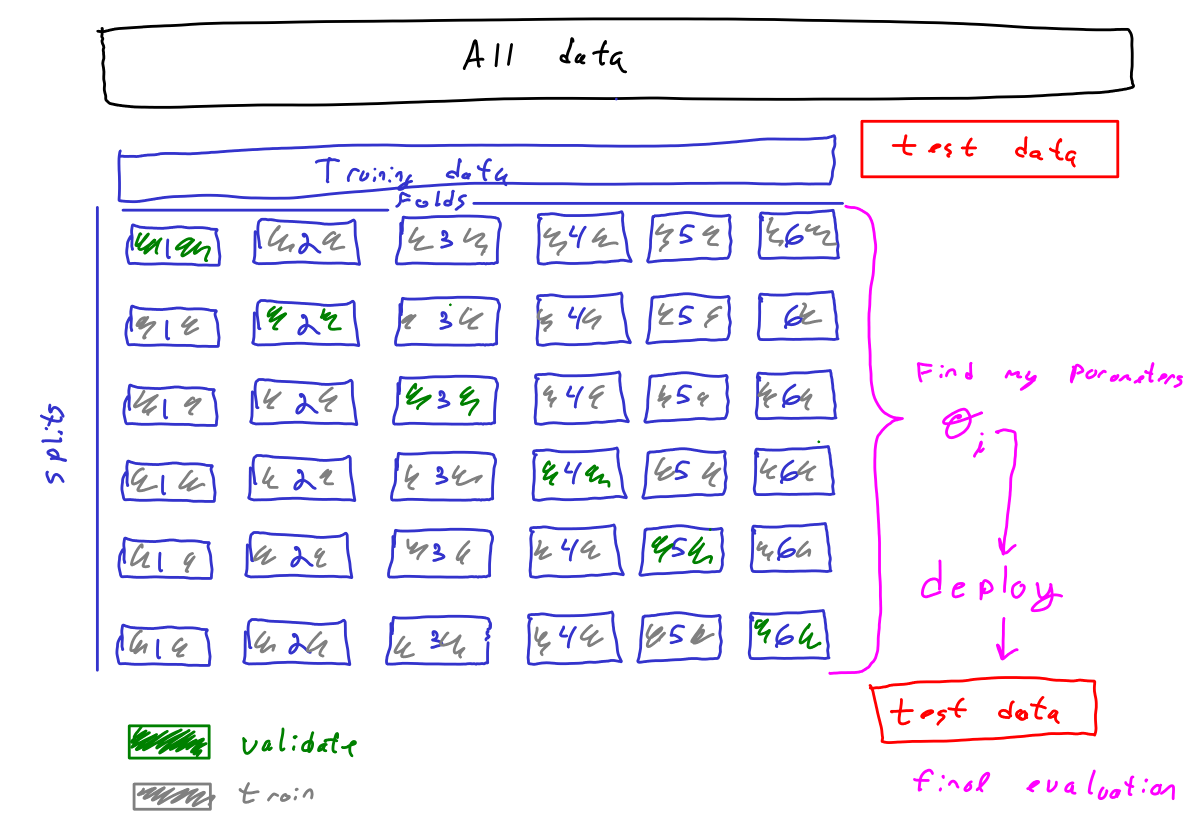
\includegraphics[width=\textwidth]
		{../figures/grid_search_cross_validation.png}
		
	\end{columns}
\end{frame}

%------------------------------------------------

\begin{frame}{Example 4.5: $k$-fold Cross-Validation}
	
	\begin{itemize}
		\item Train a binary classifier to detect the digit ``5''
		\item Repeatedly train an SGD classifier
		\item Observe variability in:
		\begin{itemize}
			\item Accuracy
			\item Precision
			\item Recall
		\end{itemize}
		
		\vspace{0.5em}
		
		\item Apply:
		\[
		\texttt{sk.model\_selection.cross\_val\_predict}
		\]
		
		\vspace{0.5em}
		
		\item Demonstrate how $k$-fold cross-validation provides more reliable performance estimates
	\end{itemize}
	
\end{frame}

%------------------------------------------------
\section{4.4~Multiclass Classification}

\begin{frame}{Multiclass Classification}
	
	Binary classifiers distinguish between:
	
	\[
	2 \text{ classes}
	\]
	
	\vspace{0.5em}
	
	Multiclass classifiers distinguish between:
	
	\[
	N > 2 \text{ classes}
	\]
	
	\vspace{0.5em}
	
	For MNIST:
	
	\[
	10 \text{ classes}
	\]
	
	corresponding to the digits:
	
	\[
	0,1,2,\ldots,9
	\]
	
	\vspace{0.5em}
	
	A common strategy is to combine multiple binary classifiers.
	
\end{frame}

%------------------------------------------------

\begin{frame}{One-vs-Rest (OvR)}
	\begin{columns}
		
		\column{0.48\textwidth}
		
		One-vs-Rest trains:
		
		\[
		N
		\]
		
		binary classifiers.
		
		\vspace{0.5em}
		
		For MNIST:
		
		\begin{itemize}
			\item 0-detector
			\item 1-detector
			\item 2-detector
			\item \ldots
			\item 9-detector
		\end{itemize}
		
		\vspace{0.5em}
		
		The class with the highest score is selected.
		
		\column{0.52\textwidth}
		\centering
		
\includegraphics[width=\textwidth]
		{../figures/one_vs_rest}
		
	\end{columns}
\end{frame}

%------------------------------------------------

\begin{frame}{One-vs-One (OvO)}
	\begin{columns}
		
		\column{0.48\textwidth}
		
		One-vs-One trains a classifier for every pair of classes.
		
		\vspace{0.5em}
		
		Number of classifiers:
		
		\[
		\frac{N(N-1)}{2}
		\]
		
		\vspace{0.5em}
		
		For MNIST:
		
		\[
		\frac{10(10-1)}{2}
		=
		45
		\]
		
		classifiers.
		
		\vspace{0.5em}
		
		The class with the most wins is selected.
		
		\column{0.52\textwidth}
		\centering
		
\includegraphics[width=\textwidth]
		{../figures/one_vs_one}
		
	\end{columns}
\end{frame}

%------------------------------------------------

\begin{frame}{Example 4.6: Multiclass Regularized Linear Classifier}
	
	\begin{itemize}
		\item Extend \texttt{SGDClassifier} to multiclass classification
		\item Compare:
		\begin{itemize}
			\item One-vs-Rest (OvR)
			\item One-vs-One (OvO)
			\item Scikit-Learn automatic strategy
		\end{itemize}
		
		\vspace{0.5em}
		
		\item Train classifiers on the MNIST dataset
		\item Measure computational cost and performance
		\item Compare strategies for distinguishing the 10 digit classes
	\end{itemize}
	
\end{frame}

%------------------------------------------------

\section{4.5~Performance Measures for Multiclass Classification}

\begin{frame}{Performance Measures for Multiclass Classification}
	
	Many of the metrics used for binary classification extend naturally to multiclass problems.
	
	\vspace{0.5em}
	
	Common evaluation tools include:
	
	\begin{itemize}
		\item Confusion matrices
		\item Accuracy
		\item Precision and recall
		\item Error analysis
	\end{itemize}
	
	\vspace{0.5em}
	
	For multiclass problems, the confusion matrix is often the most informative starting point.
	
\end{frame}

%------------------------------------------------

\begin{frame}{Multiclass Confusion Matrix}
	\begin{columns}
		
		\column{0.48\textwidth}
		
		Rows correspond to:
		
		\begin{itemize}
			\item Actual digit
		\end{itemize}
		
		\vspace{0.5em}
		
		Columns correspond to:
		
		\begin{itemize}
			\item Predicted digit
		\end{itemize}
		
		\vspace{0.5em}
		
		A good classifier has:
		
		\begin{itemize}
			\item Large values on the diagonal
			\item Small values elsewhere
		\end{itemize}
		
		\vspace{0.5em}
		
		The MNIST classifier performs well because most entries lie on the diagonal.
		
		\column{0.52\textwidth}
		\centering
		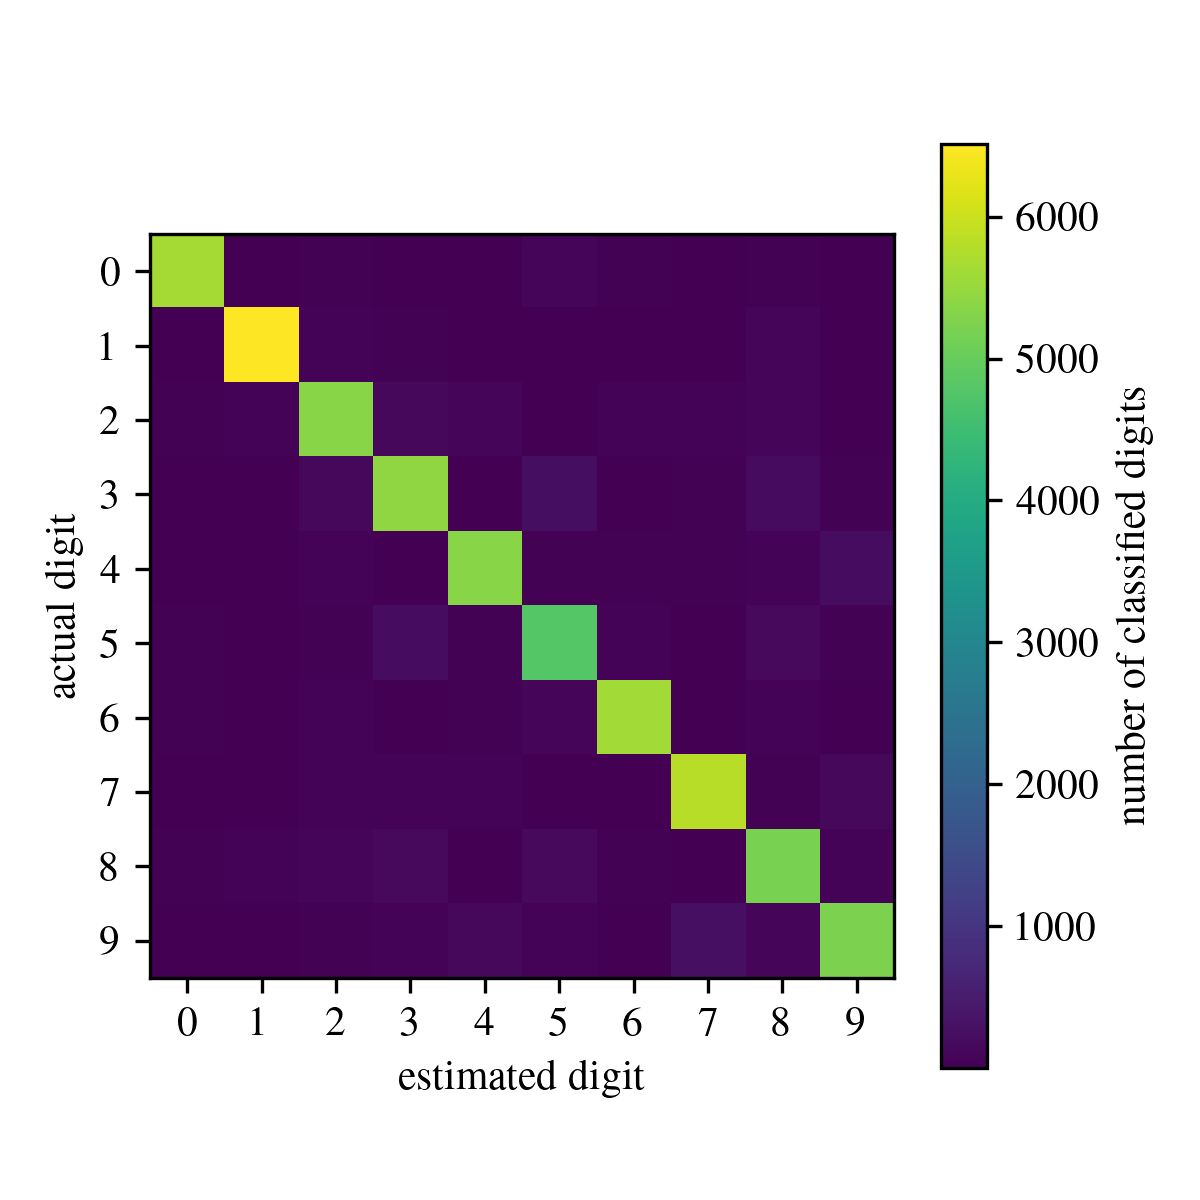
\includegraphics[width=\textwidth]
		{../figures/digit_confusion_matrix.png}
		
	\end{columns}
\end{frame}

%------------------------------------------------

\begin{frame}{Normalized Error Matrix}
	\begin{columns}
		
		\column{0.48\textwidth}
		
		To better visualize mistakes:
		
		\begin{itemize}
			\item Normalize each row
			\item Remove the diagonal entries
			\item Display only classification errors
		\end{itemize}
		
		\vspace{0.5em}
		
		This highlights which digits are most often confused.
		
		\vspace{0.5em}
		
		Brighter regions correspond to larger error rates.
		
		\column{0.52\textwidth}
		\centering
		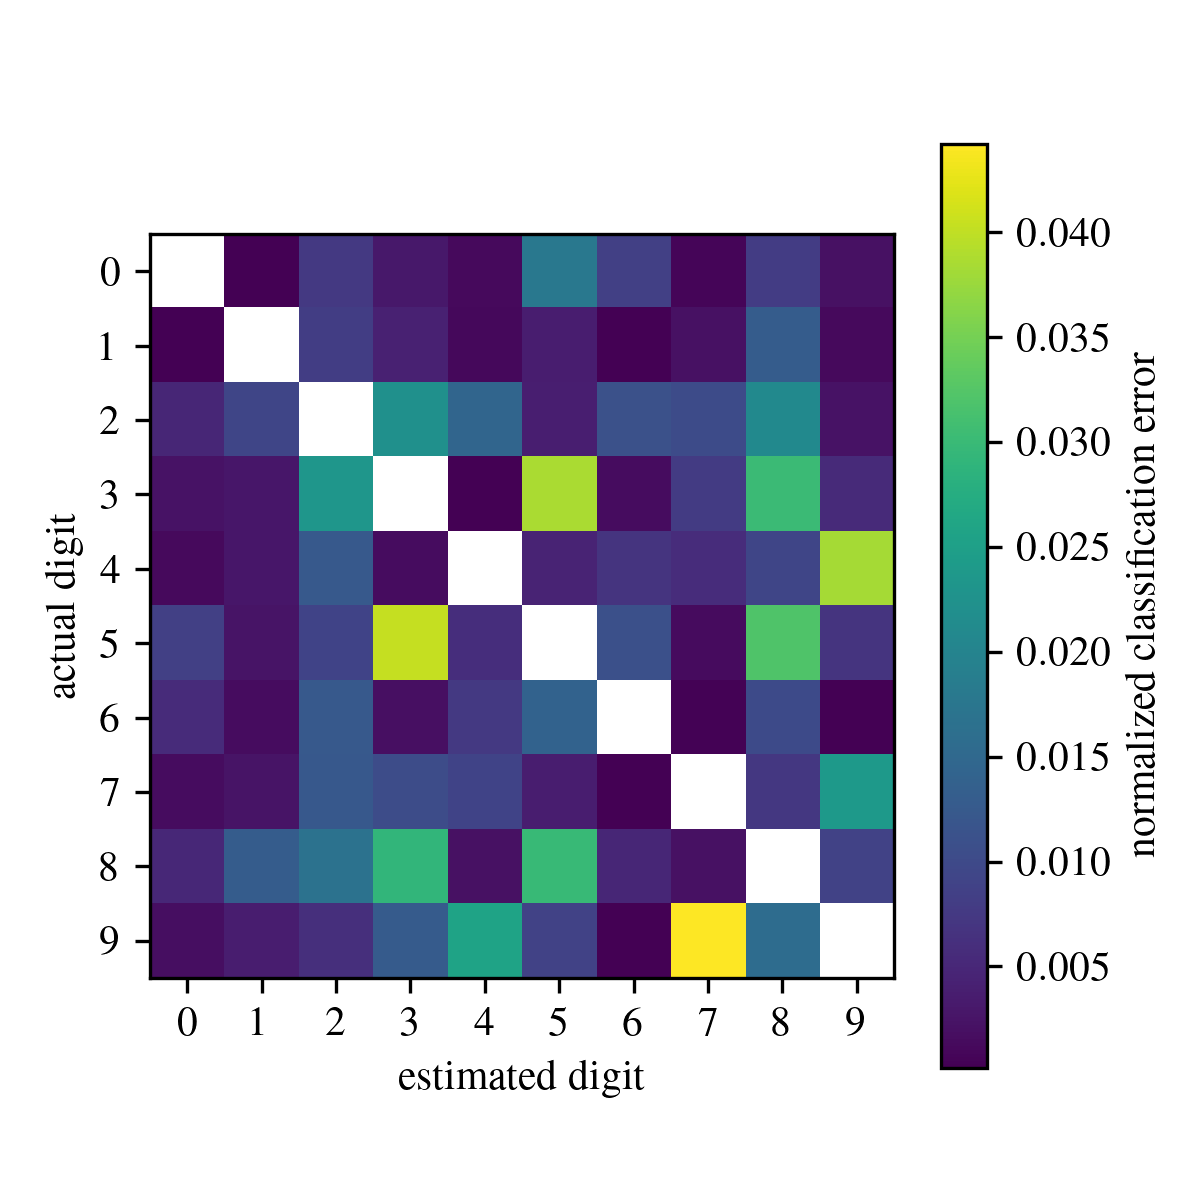
\includegraphics[width=\textwidth]
		{../figures/digit_confusion_matrix_error.png}
		
	\end{columns}
\end{frame}

%------------------------------------------------

\begin{frame}{Analyzing Individual Errors}
	\begin{columns}
		
		\column{0.48\textwidth}
		
		The classifier frequently confuses:
		
		\[
		3 \leftrightarrow 5
		\]
		
		\vspace{0.5em}
		
		Reasons:
		
		\begin{itemize}
			\item Similar handwritten shapes
			\item Small stroke differences
			\item Sensitivity to translation and rotation
		\end{itemize}
		
		\vspace{0.5em}
		
		Improvement strategies:
		
		\begin{itemize}
			\item Better preprocessing
			\item Additional features
			\item Nonlinear models
		\end{itemize}
		
		\column{0.52\textwidth}
		\centering
		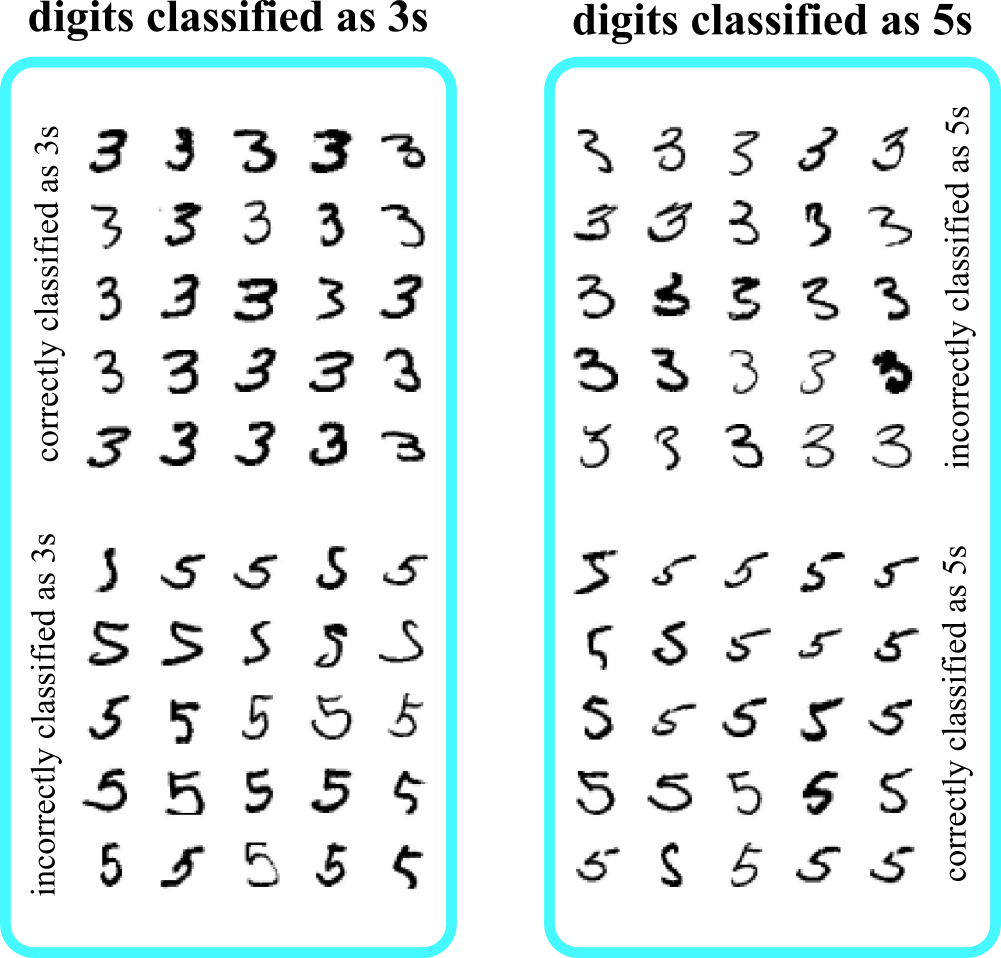
\includegraphics[width=\textwidth]
		{../figures/3s_and_5s.png}
		
	\end{columns}
\end{frame}

%------------------------------------------------

\begin{frame}{Example 4.7: Multiclass Confusion Matrix}
	
	\begin{itemize}
		\item Train a One-vs-One classifier using SGD
		\item Perform 3-fold cross-validation
		\item Construct a multiclass confusion matrix
		\item Visualize:
		\begin{itemize}
			\item Raw classification counts
			\item Normalized classification errors
		\end{itemize}
		
		\vspace{0.5em}
		
		\item Identify commonly confused digits
		\item Analyze classifier weaknesses
		\item Use the results to guide model improvements
	\end{itemize}
	
\end{frame}











\end{document}




